\documentclass[main.tex]{subfiles}

\begin{document}
   
   \chapter{Introduction}\label{chapter:introduction}
   
This is an introductory chapter. Describe what your thesis is all about here.

Use some equations:
$$H(X) = - \sum_{x\in \mathcal{X}}p(x)\log_2p(x).$$ 

Add some figures, like Fig.~\ref{fig:Fig1} or Fig.~\ref{fig:Fig2}.

\begin{figure}
      \begin{center}
	    \resizebox{5cm}{!}{\input{./figures/Fig4.pdf_t}}
      \end{center}
\caption{Illustrating the covering, packing and effective radii of the hexagonal lattice.}
\label{fig:Fig1}
\end{figure}
 
\begin{figure}
      \begin{center}
	    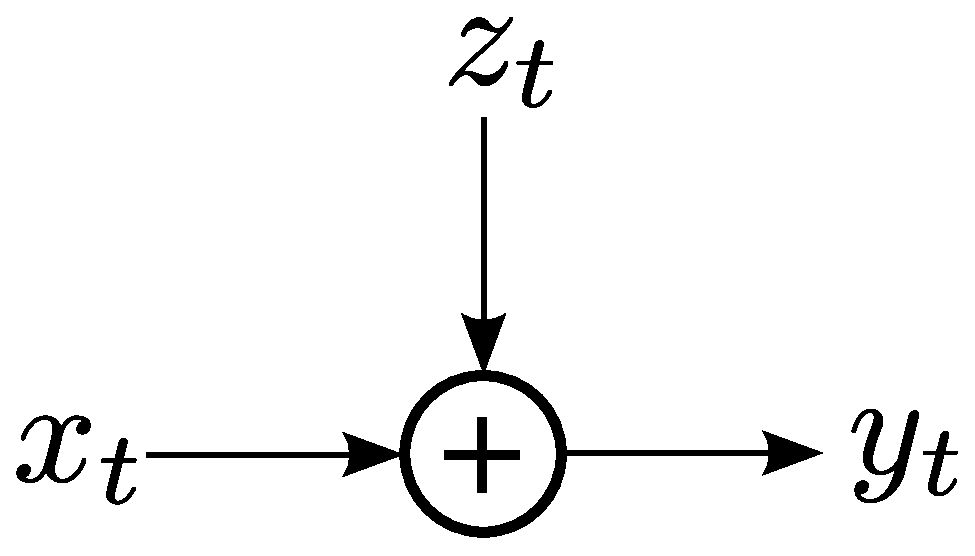
\includegraphics[width=5cm]{./figures/awgn.eps}
      \end{center}
\caption{The AWGN channel.}
\label{fig:Fig2}
\end{figure}

Cite many papers~\cite{AhlswedeCsiszar,Agrawal09}.

 \end{document}
